% domain of integration for the Madland-Nix model
\begin{center}
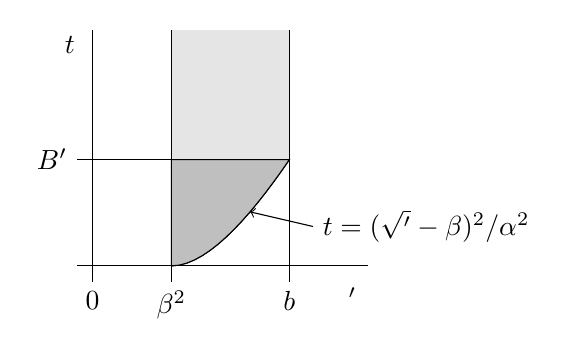
\begin{tikzpicture}
% the u_1(E) curve
\draw( 1.0 , 0.0 ) --
( 1.1 , 0.00952921463879 ) --
( 1.2 , 0.0364390799173 ) --
( 1.3 , 0.0785965992069 ) --
( 1.4 , 0.134272347041 ) --
( 1.5 , 0.202041028867 ) --
( 1.6 , 0.280711487461 ) --
( 1.7 , 0.369276151676 ) --
( 1.8 , 0.466873708001 ) --
( 1.9 , 0.572760998328 ) --
( 2.0 , 0.686291501015 ) --
( 2.1 , 0.806898603048 ) --
( 2.2 , 0.934082420647 ) --
( 2.3 , 1.06739928952 ) --
( 2.4 , 1.20645329214 ) --
( 2.5 , 1.35088935933 );
% integration regions
\filldraw[fill = gray!50]
( 1.0 , 0.0 ) --
( 1.1 , 0.00952921463879 ) --
( 1.2 , 0.0364390799173 ) --
( 1.3 , 0.0785965992069 ) --
( 1.4 , 0.134272347041 ) --
( 1.5 , 0.202041028867 ) --
( 1.6 , 0.280711487461 ) --
( 1.7 , 0.369276151676 ) --
( 1.8 , 0.466873708001 ) --
( 1.9 , 0.572760998328 ) --
( 2.0 , 0.686291501015 ) --
( 2.1 , 0.806898603048 ) --
( 2.2 , 0.934082420647 ) --
( 2.3 , 1.06739928952 ) --
( 2.4 , 1.20645329214 ) --
( 2.5 , 1.35088935933 ) --
(1, 1.35088935933 ) -- cycle;
\fill[ gray!20] ( 2.5 , 1.35088935933 ) --
(2.5, 3) -- (1, 3) --
( 1 , 1.35088935933 ) -- cycle;
% the axes and quadrature strip
 \draw(-0.2, 0) -- (3.5, 0);
 \draw(0, -0.2) -- (0, 3);
 \draw(-0.2, 1.35088935933) -- (2.5, 1.35088935933);
 \draw(1, -0.2) -- (1, 3);
 \draw(2.5, -0.2) -- (2.5, 3);
% labels
  \node [below] at (0, -0.2){0};
  \node [below] at (1, -0.2){$\beta^2$};
  \node [below] at (2.5, -0.2){$b$};
  \node [below] at (3.3, -0.15){$\Elab'$};
  \node [left] at (-0.2, 1.35){$B'$};
  \node [left] at (-0.1, 2.8){$t$};
  %legend
  \draw [<-] ( 2.0 , 0.686291501015 ) -- (2.8, 0.5);
  \node [right] at (2.8, 0.5) {$ t = (\sqrt{\Elab'} - \beta)^2/\alpha^2$};
\end{tikzpicture}
\caption{Domain of integration for $\calG_1( \beta^2, b )$ with $b > \beta^2$
in the Madland-Nix model}
\label{Fig:Madland-Nix}
\end{center} 
